\originalchapter{作业 6}
MIT 18.330, Spring 2012. 原件: Homework 6, Due Thursday April 26. 以下解答均为 AI 编写, 非官方答案.

\begin{exercise}\label{ps6-q1}
(原题 1, 7 分) 考虑混合 Neumann--Dirichlet 边值问题
$-u''=f$, $x\in[0,1]$, $u'(0)=0$, $u(1)=0$.
\begin{enumerate}[label=(\alph*)]
\item 求所有特征值 $\lambda_n$ 和特征函数 $v_n$, 使
$-v_n''=\lambda_nv_n$, $v_n'(0)=0$, $v_n(1)=0$.
手画前三个特征函数. 提示: 取正弦或余弦, 由边界条件确定.
\item 取 $x_j=jh$, $h=1/N$, $j=0,\ldots,N-1$, 用基本二阶差分离散二阶导数. 为简单起见, 将 Neumann 条件离散为 $(U_1-U_0)/h=0$.
写出离散系统的矩阵, 给出创建矩阵的 MATLAB 代码, 称它为 $T$.
\item 对适当的大 $N>100$, 用 MATLAB 的 \texttt{eig} 求 $T$ 的特征值与特征向量, 画前三个特征向量, 与连续预测比较. 提示: 特征值输出未必递增, 要同步排序特征值和特征向量.
\item 取 $f=1$, 离散成 $F_j=1$, 用 MATLAB 的反斜杠解 $TU=F$. 对不同 $N$ 绘制误差的双对数图, 误差取
$\|u-U\|_h=[h\sum_{j=0}^{N-1}(u(x_j)-U_j)^2]^{1/2}$.
提示: 可用很细网格的数值解作参考; 两网格应嵌套以便比较.
\item 原件称, 因边界条件仅一阶精度, 上述范数下局部截断误差为 $O(h)$. 要推出同一范数下全局误差也为 $O(h)$, $T$ 应满足什么性质?
\end{enumerate}
\end{exercise}
\begin{solution}
(a) 乘以 $v$ 并分部积分得 $\lambda\int_0^1v^2=\int_0^1(v')^2$, 因边界项为零, 非零特征函数不可能有 $\lambda\le0$ (等号会使 $v$ 为常数再由右端值为零排除).
因此 $v=A\cos(\sqrt\lambda x)+B\sin(\sqrt\lambda x)$, 左端导数条件给出 $B=0$, 右端给出
$\sqrt\lambda=(n+1/2)\pi$, $n=0,1,\ldots$.
于是 $\lambda_n=(n+1/2)^2\pi^2$, $v_n(x)=\cos((n+1/2)\pi x)$, 可乘任意非零常数. 下图虚线即前三个余弦, 依次有零、一、两个内部零点.

(b) 整理注: 若保留边界方程的一整行, 其右端必须是 $0$, 不能在该行也取 $F_0=1$; 而对包含边界行的矩阵直接用普通 \texttt{eig} 比较微分算子谱, 结果会依赖边界行的缩放. 为同时明确 (c)、(d), 本解答先消去 $U_0=U_1$, 将独立未知量取为
$W=(U_1,\ldots,U_{N-1})^T$, 并将所得矩阵称为 $T$. 最后恢复 $U_0=U_1$. 这保留全部题给网格点和边界条件, 不在边界处额外施加 $-u''=f$.
\[
T=\frac1{h^2}\begin{pmatrix}
1&-1&&\\
-1&2&-1&\\
&\ddots&\ddots&\ddots\\
&&-1&2
\end{pmatrix}_{(N-1)\times(N-1)}.
\]
完整未消元系统的第一行为 $(-U_0+U_1)/h=0$, 其余行为 $(-U_{j-1}+2U_j-U_{j+1})/h^2=F_j$, $1\le j\le N-1$, 最后一行代入 $U_N=0$. MATLAB 核心代码为
\begin{verbatim}
h=1/N; m=N-1;
T=diag(2*ones(m,1))+diag(-ones(m-1,1),1) ...
  +diag(-ones(m-1,1),-1);
T(1,1)=1; T=T/h^2;
[V,D]=eig(T); [lam,idx]=sort(diag(D)); V=V(:,idx);
W=T\ones(m,1); U=[W(1);W];
\end{verbatim}

(c) 对 $m=N-1$, 特征向量在独立节点上可取
$w_j=\cos((j-1/2)\theta)$, $1\le j\le m$;
左端虚拟值 $w_0=w_1$, 右端 $w_{m+1}=0$, 故
$\theta_n=(n+1/2)\pi/(N-1/2)$,
$\lambda_{n,h}=4h^{-2}\sin^2(\theta_n/2)$, $0\le n\le N-2$.
当 $h\to0$ 时固定编号的特征值趋向 (a) 的值.
实际取 $N=256$, 前三个为 $2.4770598945,22.2929773029,61.9218162242$, 连续值为
$2.4674011003,22.2066099025,61.6850275068$.
\begin{center}
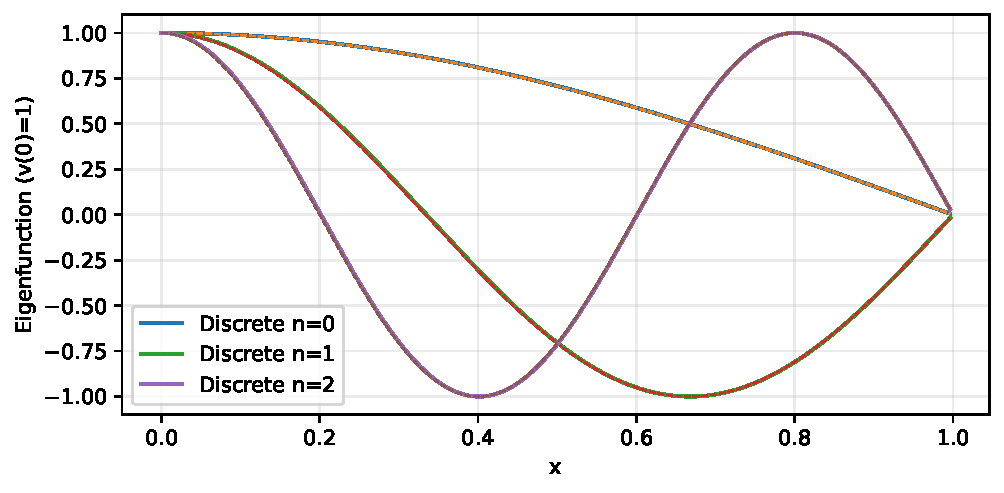
\includegraphics[width=.88\linewidth]{figures/assessments/ps6_eigenvectors.pdf}
\end{center}
脚本同步取前三个递增特征值及对应向量, 恢复 $U_0=U_1$, 并归一化左端值为 $1$. 实际 Python 使用对称三对角特征求解器; 上述 MATLAB 代码给出题目要求的 \texttt{eig} 等价做法.

(d) 真解为 $u(x)=(1-x^2)/2$. 消元系统的各内部右端确为 $1$, 可直接解析核对
$U_j=(1-x_j^2)/2-(h/2)(1-x_j)$, $0\le j\le N$, 它满足 $U_0=U_1$, $U_N=0$ 和所有内部差分方程. 因而
\[
\|u-U\|_h=\frac h2\left[h\sum_{j=0}^{N-1}(1-jh)^2\right]^{1/2}
\sim\frac{h}{2\sqrt3}.
\]
实际 $N=16,32,\ldots,4096$ 的误差拟合斜率约 $1.001$, 与一阶一致. 采用解析真解避免参考网格误差污染.
\begin{center}
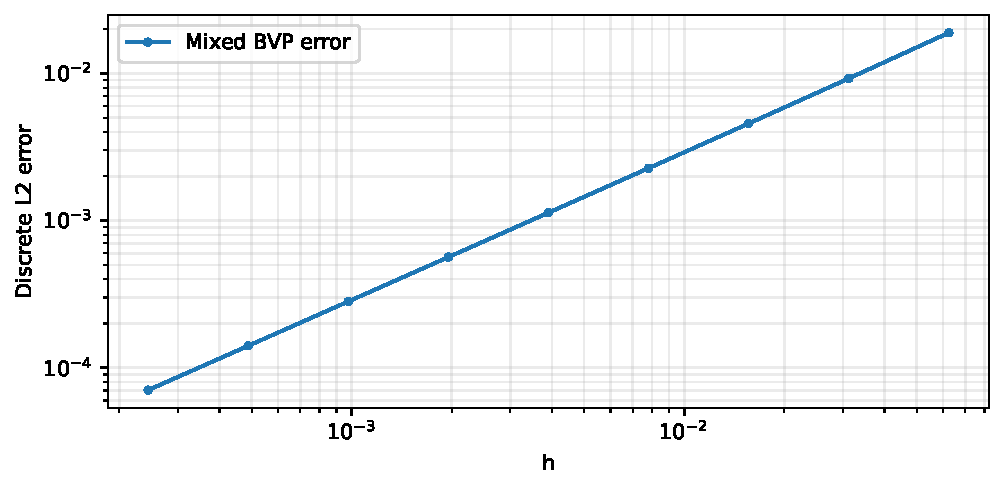
\includegraphics[width=.85\linewidth]{figures/assessments/ps6_convergence.pdf}
\end{center}

(e) 一般若 $\tau=T u_{\mathrm{grid}}-F$, $e=u_{\mathrm{grid}}-U$, 则 $Te=\tau$. 从 $\|\tau\|_h=O(h)$ 推出同阶全局误差的充分性质是稳定性: 诱导范数 $\|T^{-1}\|_{h\to h}\le C$ 一致于 $h$.
对本题对称正定的消元矩阵, 该范数等于 $1/\lambda_{0,h}$, 由 (c) 的公式有统一正下界 (例如 $\lambda_{0,h}\ge1$), 所以一致有界.

但原件“局部截断误差在同一二次范数中为 $O(h)$”并未随边界方程形式自动成立. 对 (b) 的明确消元约定和本题二次真解, $\tau=(1/2,0,\ldots,0)^T$, 在内部节点范数中是 $\sqrt h/2=O(h^{1/2})$. 单纯范数估计只给 $O(h^{1/2})$, 不能由它假证一阶. 实际
$(T^{-1}e_1)_j=h(1-x_j)$, 直接给出 (d) 的 $O(h)$ 全局误差; 恢复边界点后仍同阶. 因此保留原问并回答其所需的稳定性质, 同时明确原件关于局部范数的不足, 不把不同边界行缩放混成一个无条件结论.
\end{solution}

\begin{exercise}\label{ps6-q2}
(原题 2, 2 分) 考虑 Neumann 问题
$-\frac{\dd}{\dd x}[(1+x^2)u']=f$,
$x\in[0,1]$, $u'(0)=u'(1)=0$.
\begin{enumerate}[label=(\alph*)]
\item 证明 $f=1$ 时无解. 提示: 两端积分.
\item 求一个保证存在解的 $f$ 的条件.
\end{enumerate}
\end{exercise}
\begin{solution}
(a) 积分左端为 $-[(1+x^2)u']_0^1=0$, 右端为 $1$, 矛盾.
(b) 对连续 $f$, 充要条件为 $\int_0^1f(x)\dd x=0$.
必要性同 (a). 若满足条件, 令
$u'(x)=-[\int_0^x f(t)\dd t]/(1+x^2)$, 再取
\[
u(x)=C-\int_0^x\frac{\int_0^s f(t)\dd t}{1+s^2}\dd s.
\]
则 $u\in C^2$, 两端导数为零, 并满足微分方程. 常数 $C$ 任意, 体现纯 Neumann 问题的非唯一性.
\end{solution}

\begin{exercise}\label{ps6-q3}
(原题 3, 1 分) 设 $A=\left(\begin{smallmatrix}2&a\\1&0\end{smallmatrix}\right)$.
\begin{enumerate}[label=(\alph*)]
\item 对哪些 $a$ 可逆?
\item 不计算特征值和特征向量, 求使 $A$ 存在特征向量的标准正交基的 $a$, 并解释.
\end{enumerate}
\end{exercise}
\begin{solution}
(a) $\det A=-a$, 故当且仅当 $a\ne0$ 可逆.
(b) 对实标准正交特征基, $A=QDQ^T$ 必为对称矩阵, 所以 $a=1$ 是必要条件; 此时矩阵实对称, 由谱定理也充分.
若允许复正交基, 矩阵必须正规; 比较 $AA^*$ 与 $A^*A$ 的非对角元同样给出 $2=2a$, 仍只有 $a=1$.
\end{solution}
